%-------------------------------------------------------
\documentclass[aspectratio=149]{beamer}
\usepackage{lmodern}
\usefonttheme[onlymath]{serif}
\usetheme{Hannover}
% \usetheme{Singapore}
% \usetheme{CambridgeUS}
% \usetheme{Boadilla}
% \usetheme{Madrid}
% \usetheme{Szeged}
% \usetheme{Frankfurt}
\colorlet{beamer@blendedblue}{teal!35!black}
% \usecolortheme{beaver}
\setbeamertemplate{navigation symbols}{}

%\hypersetup{pdfpagemode=FullScreen}

\usepackage[mode=build]{standalone}
\usepackage[absolute,overlay]{textpos}
\usepackage[utf8]{inputenc}
\usepackage[spanish]{babel}
\usepackage{hyperref}
\usepackage{tikz}
\usepackage{graphicx}
\usepackage{booktabs}
\usepackage{caption}
\usepackage[rightcaption]{sidecap}
\usepackage{caption}
\usepackage{makecell}
% \usepackage{emoji}
\graphicspath{{../images/}}

\usepackage{apacite}
%\usepackage{natbib}
\usepackage{etoolbox}
\renewenvironment{APACrefURL}[1][]{}{}
\AtBeginEnvironment{APACrefURL}{\renewcommand{\url}[1]{}}
\renewcommand{\doiprefix}{doi:~\kern-1pt}

\bibliographystyle{apacite}

\title{Tasa de matriculación }
\subtitle{de alumnos universitarios pregrado}
\author{Alejandro Acosta León}

\date{\today}

% \logo{
% \includegraphics[width=2.5cm]{C:/Users/alejo/OneDrive - Universidad de Las Américas/Ico/economia-logo.png}
% }


\begin{document}
%-------------------------------------------------------
\maketitle

\section{Introducción}
\begin{frame}
	\frametitle{El proceso de admisión}
	\centering
	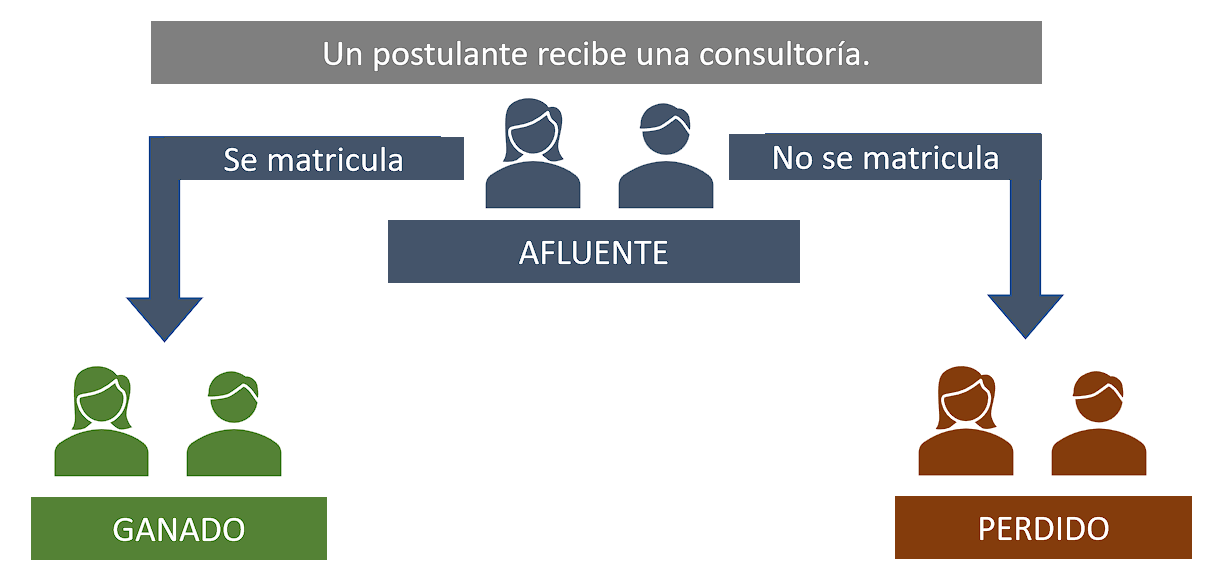
\includegraphics[width=\textwidth]{intro.png} \\
	\vspace{0.3cm}
	$conv = \frac{Ganados}{Afluentes}$
\end{frame}

\section{Datos}
\begin{frame}
	\frametitle{Datos e imputación}
	\centering
	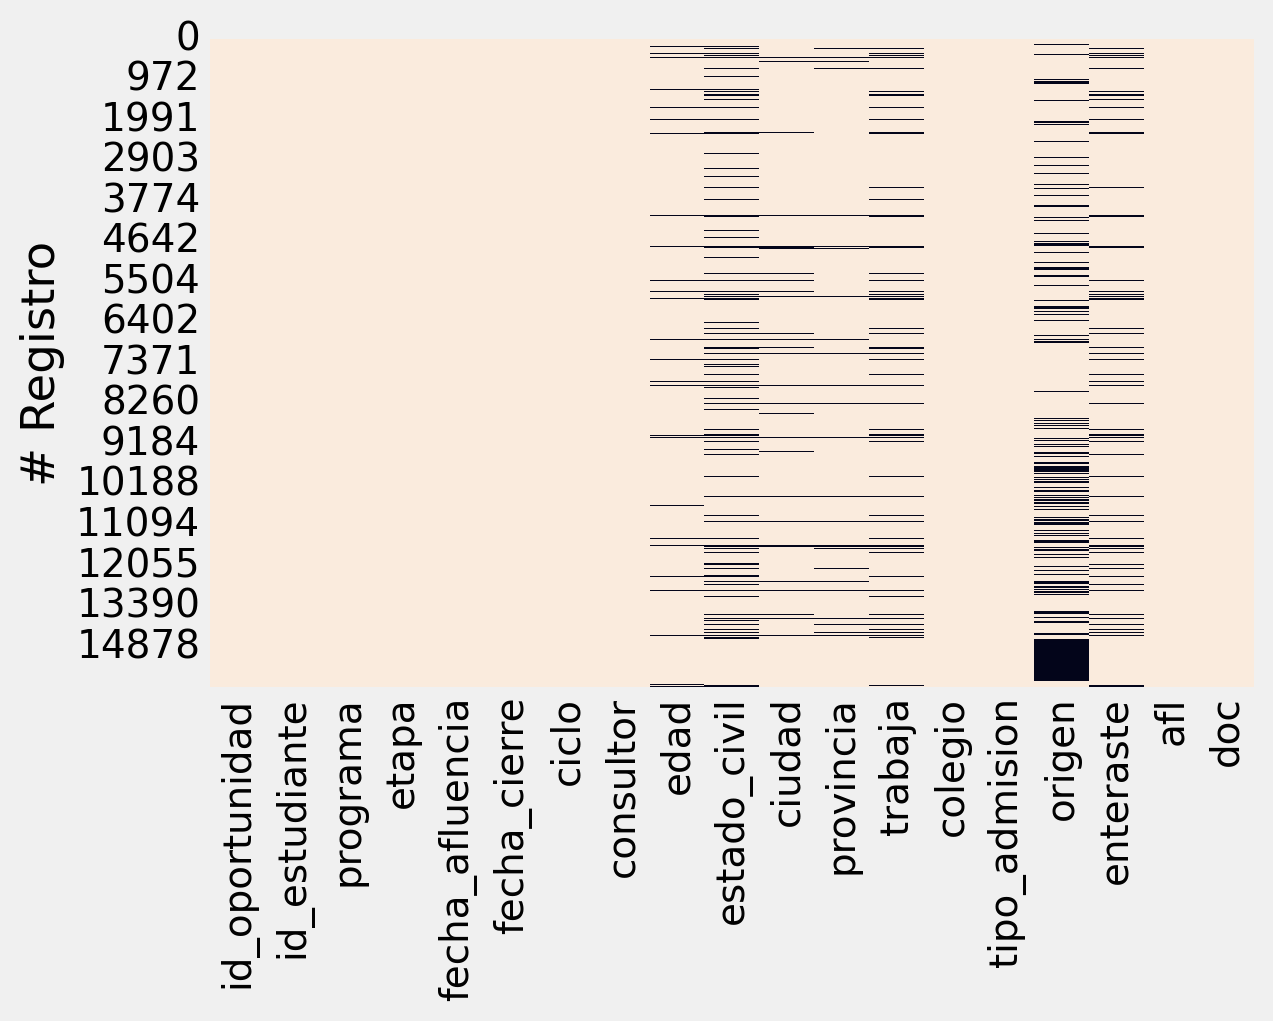
\includegraphics[width=0.70\textwidth]{missings.png} \\
	Tras la limpieza se tienen 12626 Observaciones, 9.3\% de registros con valores perdidos.
\end{frame}

\subsection{Var. Objetivo}
\begin{frame}
	\frametitle{Variable objetivo}
	\centering
	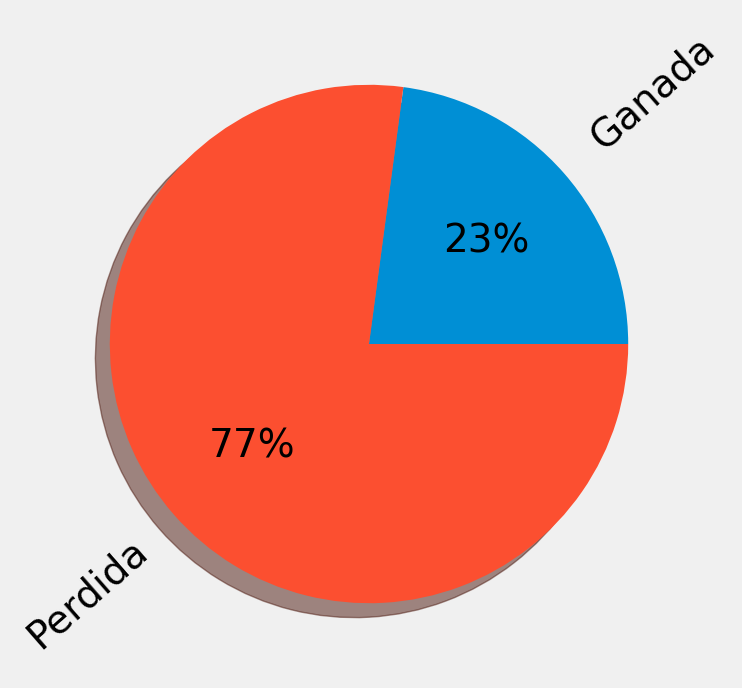
\includegraphics[width=0.7\textwidth]{conversion.png} \\
\end{frame}


\subsection{Var. explicativas}
\begin{frame}
	\frametitle{Variables explicativas}
	\framesubtitle{Glosario}
	\underline{\textbf{Variables del proceso de admisión:}}
	\begin{enumerate}
		\item \textbf{Programa}: código del programa académico.
		\item \textbf{Ciclo}: tiempo en días transcurrido entre la fecha de afluencia y la de cierre.
		\item \textbf{Consultor}: código del consultor que le atendió.
		\item \textbf{Tipo\_Admision}: Normal o convalidado.
		\item \textbf{Enteraste}: ¿cómo te enteraste de la universidad?
	\end{enumerate}
	
	\underline{\textbf{Variables demográficas del postulante}}
	\begin{enumerate}
		\item \textbf{Estado\_Civil}
		\item \textbf{Edad}
		\item \textbf{Provincia}
		\item \textbf{Trabaja}: 1 si trabaja, 0 caso contrario.
		\item \textbf{Colegio}: código del colegio donde estudió.
	\end{enumerate}
\end{frame}

\section{Estadística descriptiva}
\subsection{Ciclo}
\begin{frame}
	\frametitle{Hallazgos importantes}
	\framesubtitle{Ciclo}
	\begin{columns}
		\begin{column}{0.55\textwidth}
			\centering
			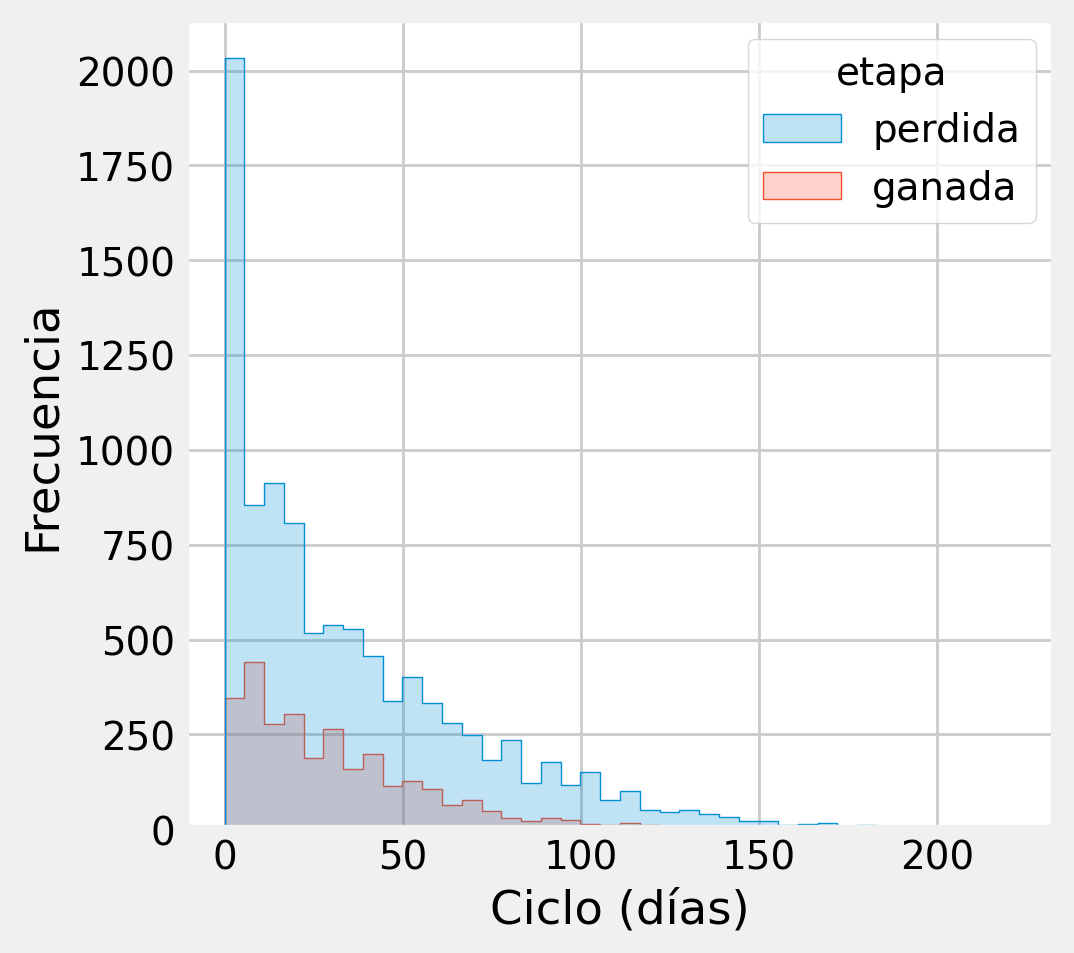
\includegraphics[width=\textwidth]{ciclo-histograma.png} \\
		\end{column}
		\begin{column}{0.46\textwidth}
			\centering
			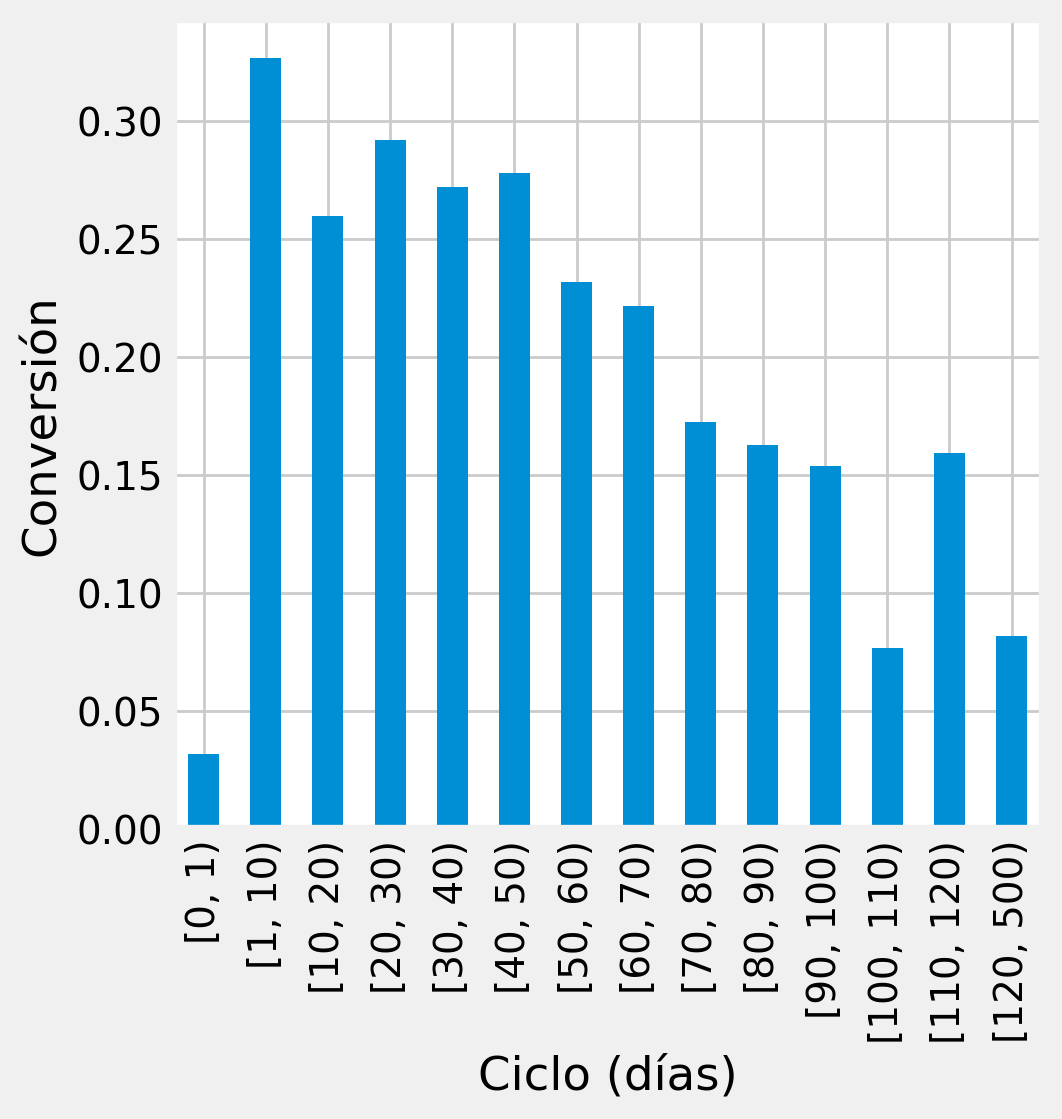
\includegraphics[width=\textwidth]{conversion-ciclo.png} \\
		\end{column}
	\end{columns}
	\vspace{0.5cm}
	Un ciclo corto (¡pero no tan corto!) incrementa la probabilidad de matriculación.
\end{frame}

\subsection{Colegio}
\begin{frame}
	\frametitle{Hallazgos importantes}
	\framesubtitle{Colegio}
	\begin{columns}
		\begin{column}{0.52\textwidth}
			\centering
			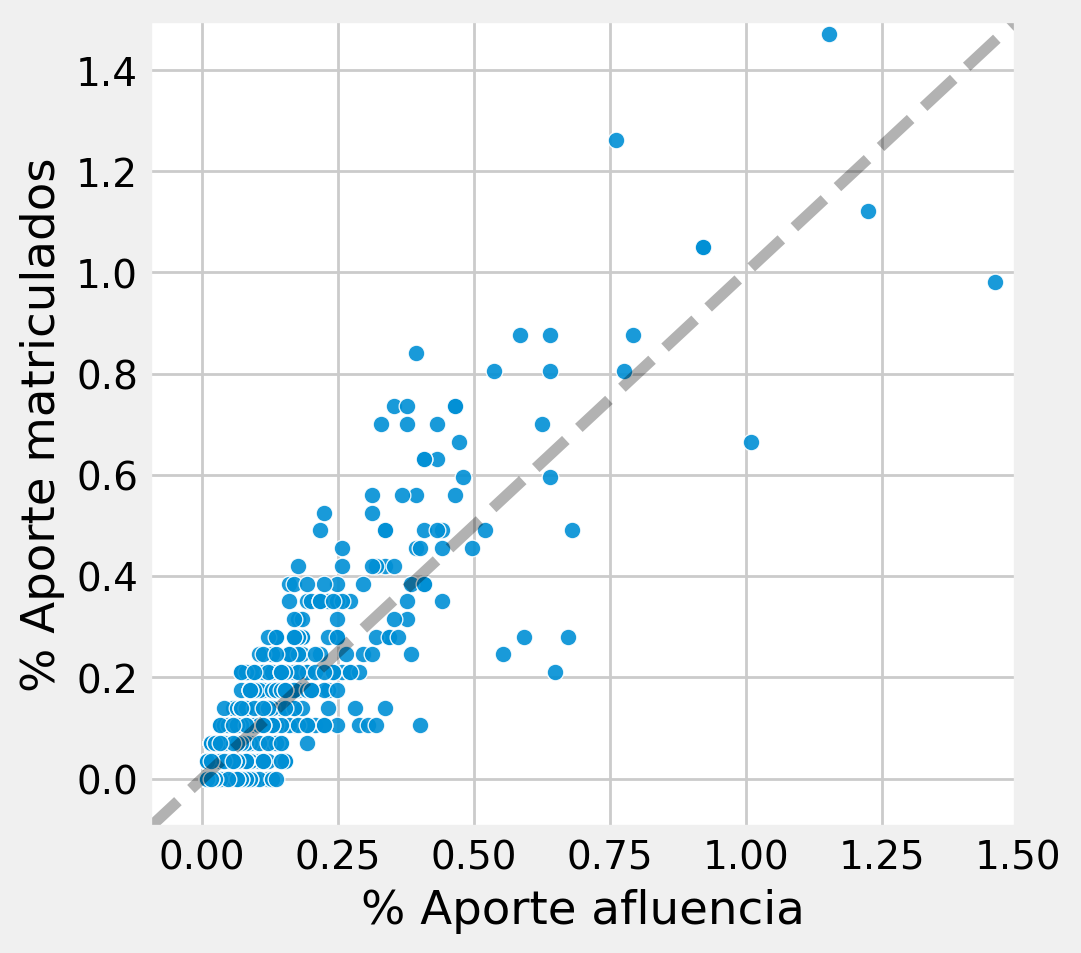
\includegraphics[width=\textwidth]{colegios.png} \\
		\end{column}
		\begin{column}{0.52\textwidth}
			\centering
			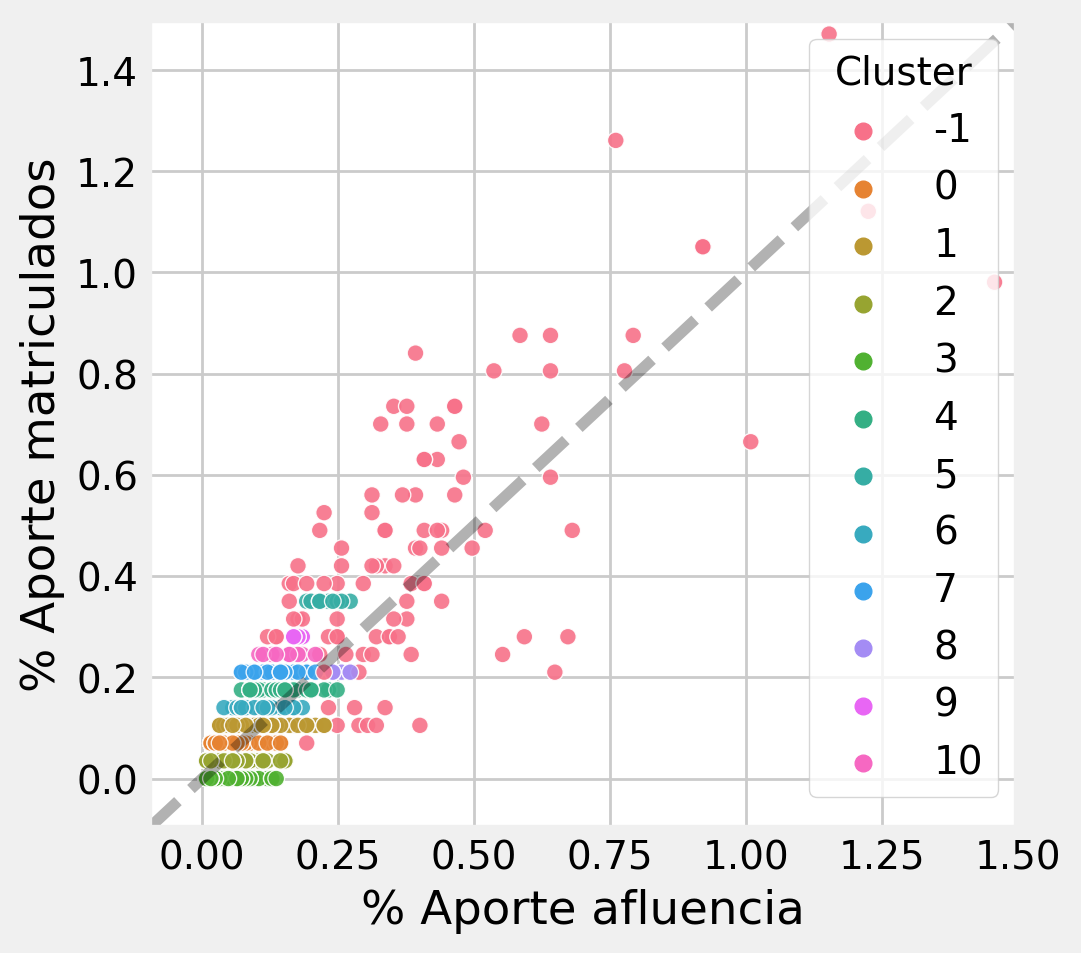
\includegraphics[width=\textwidth]{colegios-cluster.png} \\
		\end{column}
	\end{columns}
	\vspace{1cm}
	Los colegios comparten características respecto al aporte en afluencia y matriculación.
\end{frame}

\section{Modelos}
\begin{frame}
	\frametitle{Modelos}
	Ya que la variable objetivo existe en el dataset y es binaria, se requiere un modelo supervisado de clasificación. \\
	\begin{itemize}
		\item Ratio de 70\% para entrenamiento. 
		\item El número de estimadores óptimo se encontrará mediante un Grid Search.
	\end{itemize}
	
	\noindent\rule{10cm}{0.4pt}

	\begin{block}{Random Forest}
		N-Estimators: 800
	\end{block}

	\begin{block}{XGBoost}
		N-Estimators: 200
	\end{block}
\end{frame}


\section{Resultados}
\subsection{Accuracy}
\begin{frame}
	\frametitle{Resultados}
	\framesubtitle{Accuracy del modelo}
	\begin{columns}
		\begin{column}{0.50\textwidth}
			\centering
			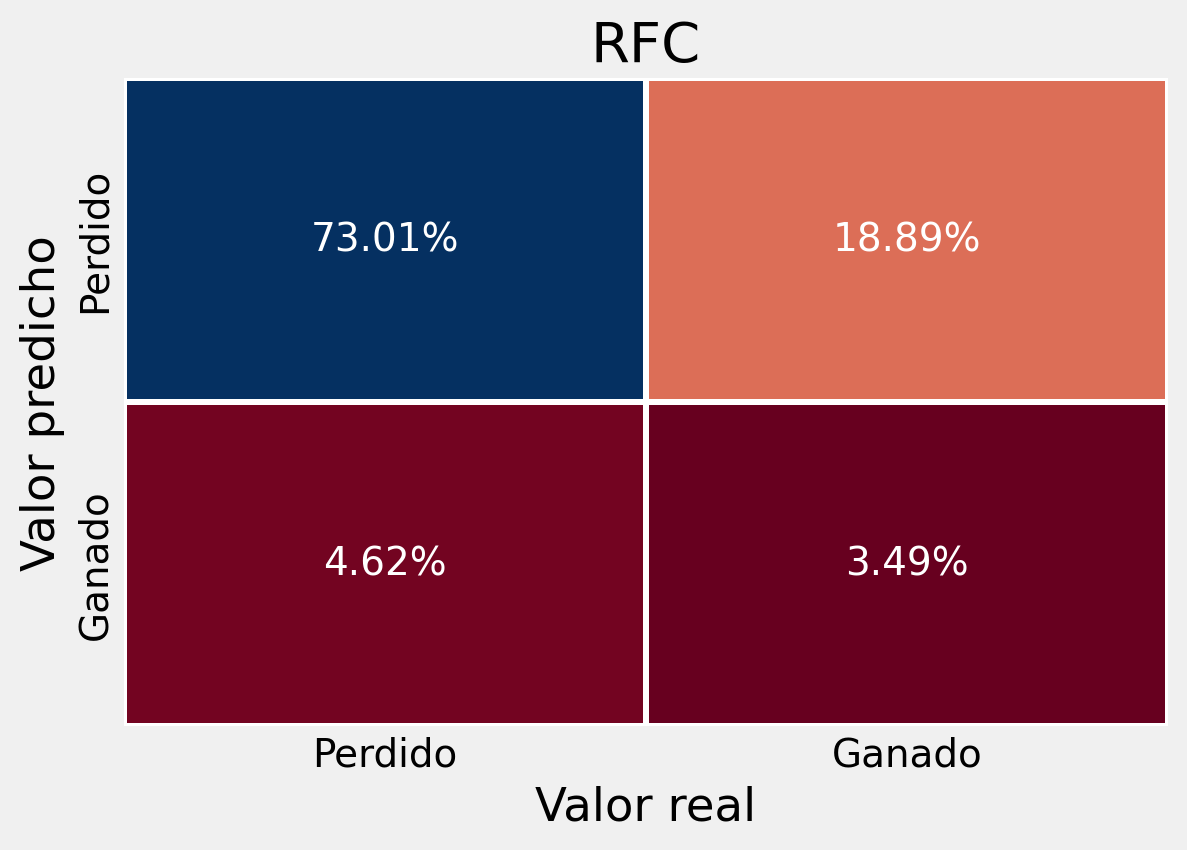
\includegraphics[width=\textwidth]{rfc-cm.png} \\
			\textbf{Accuracy: 76\%} \\
			\textbf{Sensitivity: 16\%} \\
			\textbf{Specificity: 94\%}

		\end{column}
		\begin{column}{0.50\textwidth}
			\centering
			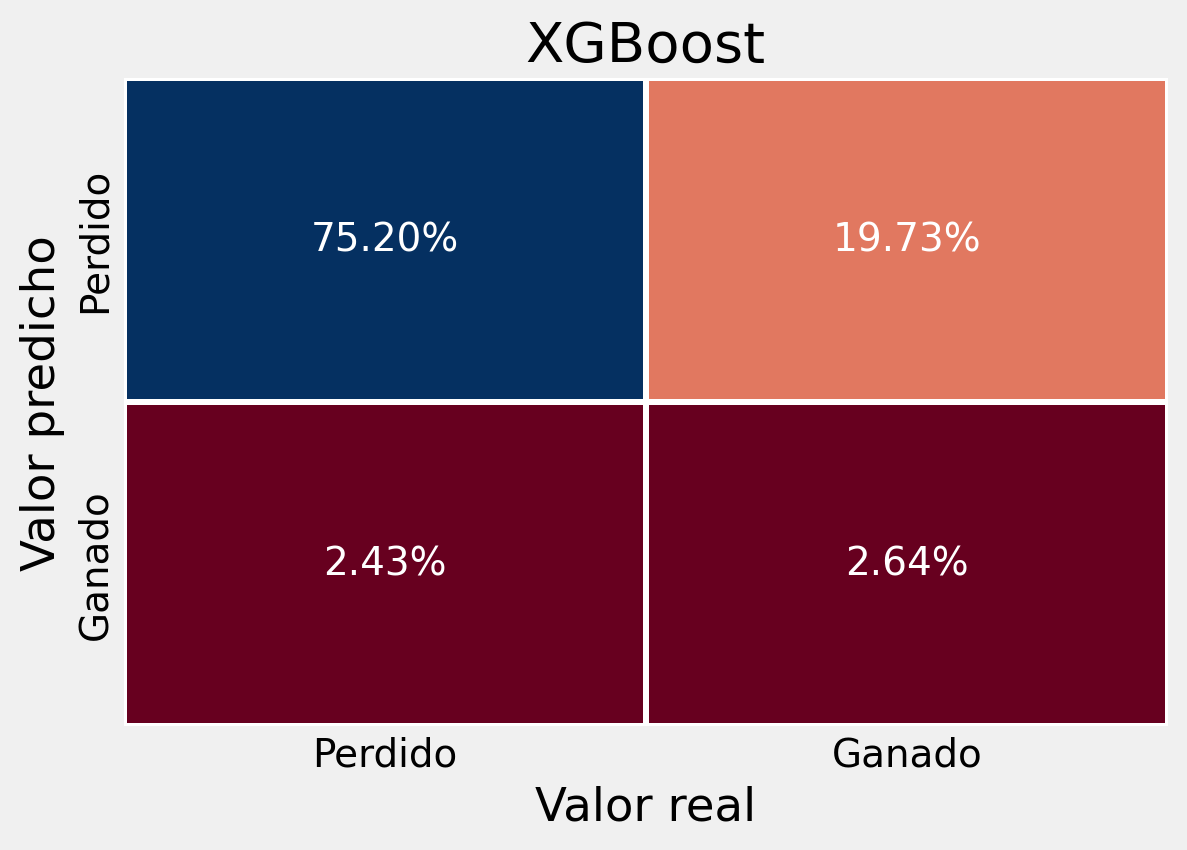
\includegraphics[width=\textwidth]{xgb-cm.png} \\
			\textbf{Accuracy: 77\%} \\
			\textbf{Sensitivity: 12\%} \\
			\textbf{Specificity: 97\%}

		\end{column}
	\end{columns}
	\vspace{0.3cm}
	El modelo XGBoost mejora la predicción de perdidos pero empeora la predicción de ganados.
\end{frame}

\subsection{Importancia variables}
\begin{frame}
	\frametitle{Resultados}
	\framesubtitle{Importancia de la variable}
	\begin{columns}
		\begin{column}{0.50\textwidth}
			\centering
			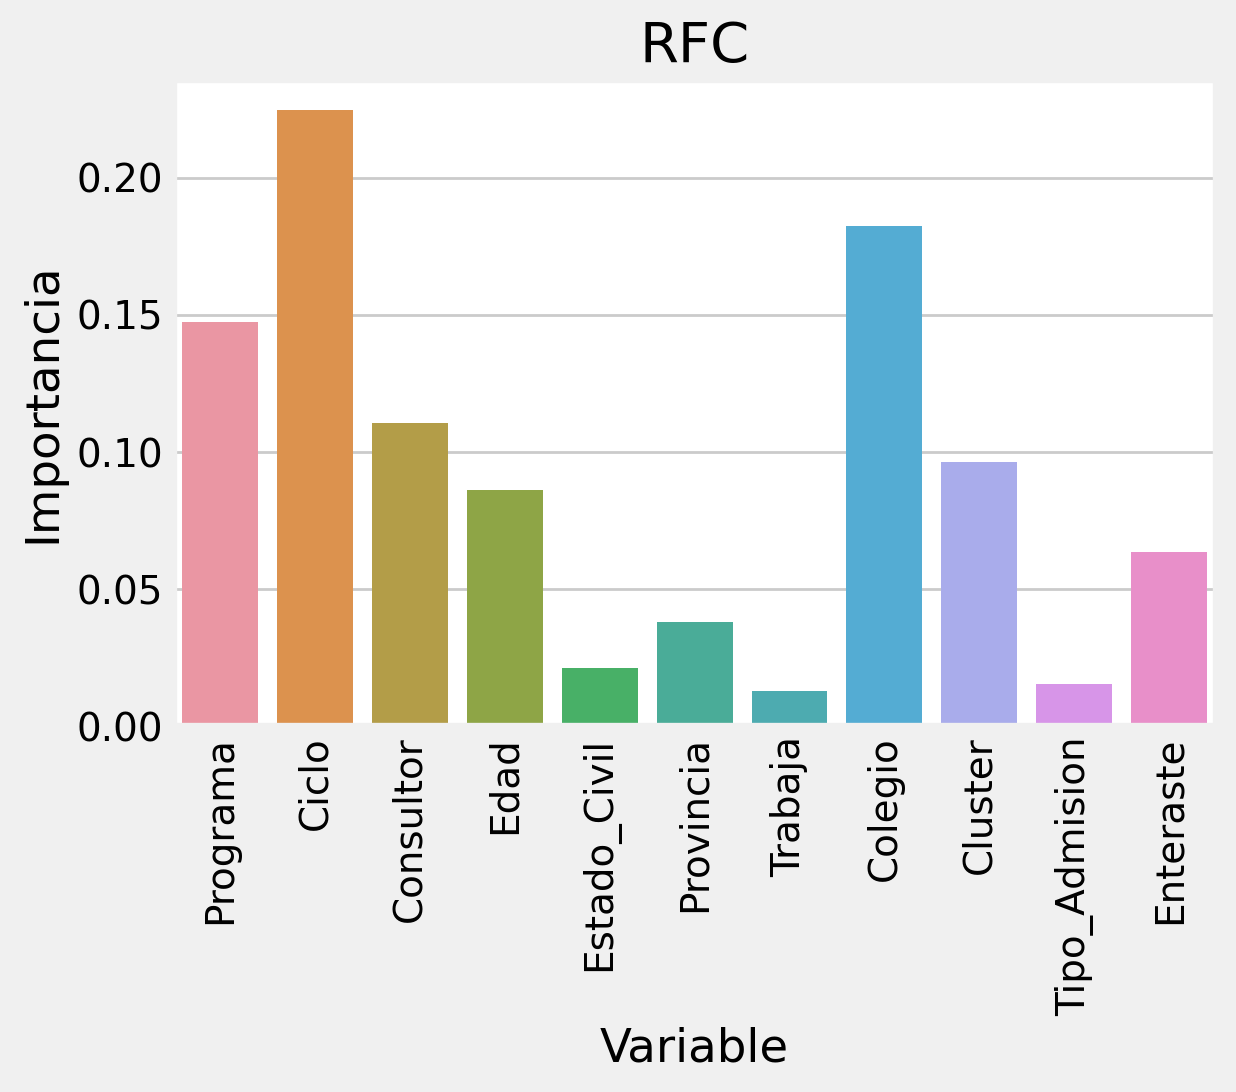
\includegraphics[width=\textwidth]{rfc-importancia.png} \\

		\end{column}
		\begin{column}{0.50\textwidth}
			\centering
			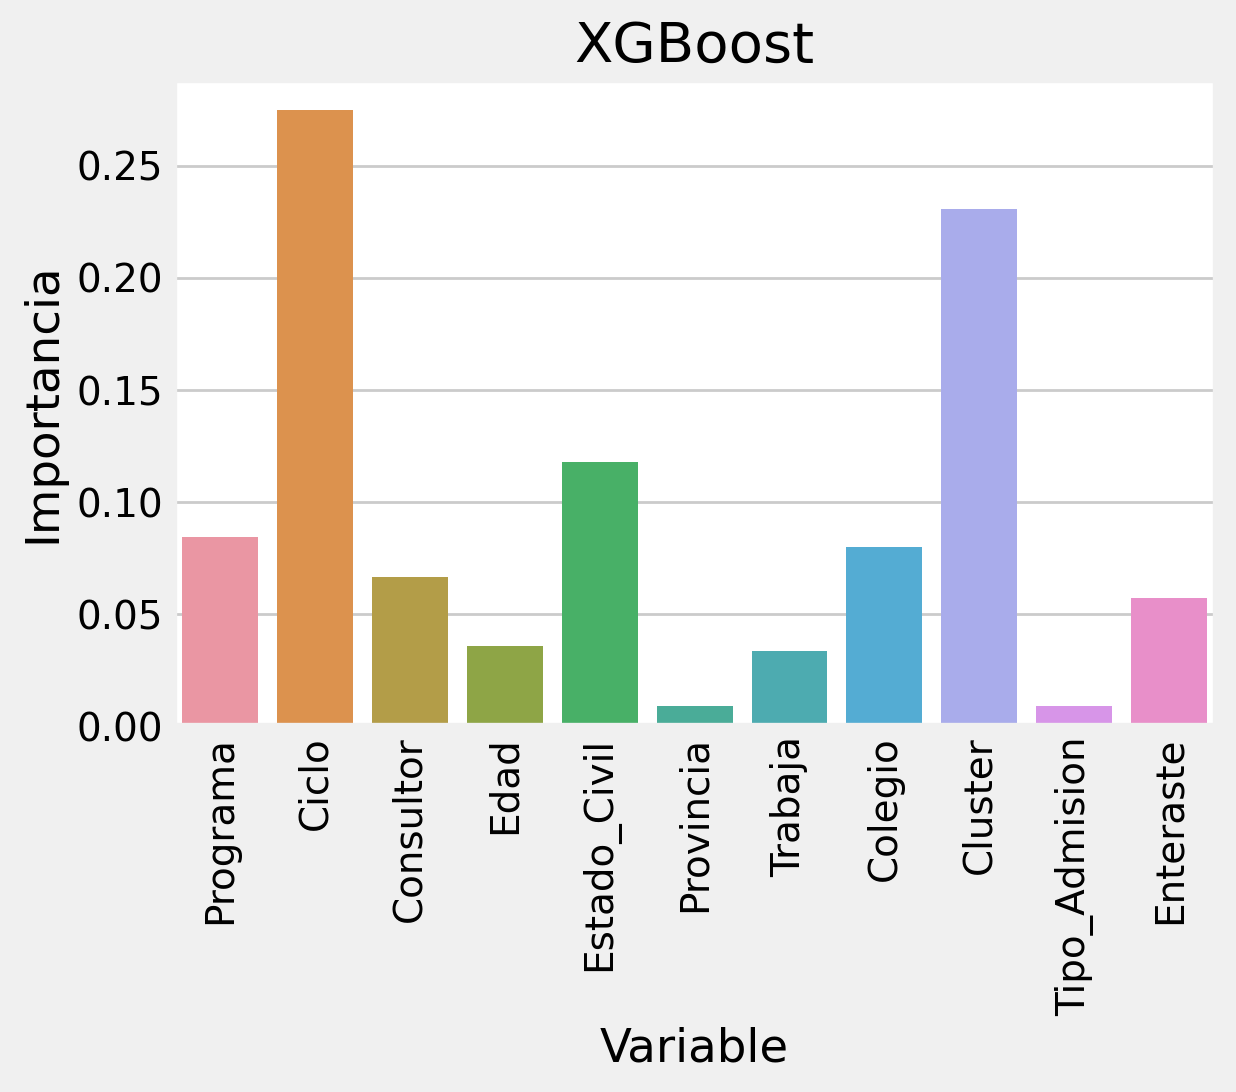
\includegraphics[width=\textwidth]{xgb-importancia.png} \\

		\end{column}
	\end{columns}
	\vspace{0.3cm}
	Ciclo y colegio son las variables mas importantes.
\end{frame}

\section{Conclusiones}
\begin{frame}
	% \frametitle{Conclusiones}
	\vfill
	\hfill {\hskip-1.8em\usebeamerfont{frametitle}\usebeamercolor[fg]{frametitle} Conclusiones}
	\vfill
	\begin{itemize}
		\item ¡El ciclo de venta importa!
		\item Mantener buenas relaciones y convenios con colegios claves puede mejorar la conversión.
		\item La provincia aparentemente no es relevante, pero esto puede deberse a que Pichincha está sobre representado.
	\end{itemize}

	\vfill
	\hfill {\hskip-1.8em\usebeamerfont{frametitle}\usebeamercolor[fg]{frametitle} Siguientes pasos}
	\vfill

	\begin{itemize}
		\item La variable objetivo podría cambiar al \% de beca ofrecida.
		\item De esta forma se podría estimar una especie de ''elasticidad'' del postulante.
		\item Es posible integrar el modelo predictivo CRM, de tal forma que el consultor tenga en tiempo real una recomendación de beca y probabilidad de matriculación basado a las características del postulante.
	\end{itemize}

\end{frame}

%-------------------------------------------------------
\end{document}








% \begin{document}
% \maketitle

% \section{Introducción}
% \begin{frame}
% 	\frametitle{En esta sesión revisaremos:}
% 	\underline{\textbf{Conceptos}}
% 		\begin{itemize}
% 			\item ¿Qué es Power BI? ¿Cuándo usarlo y cuándo no?
% 			\item Elementos básicos de Power BI desktop
% 			\item Los dos lenguajes de Power BI: DAX y M
% 		\end{itemize}
% 		\underline{\textbf{Práctica}}
% 		\begin{itemize}
% 			\item Importación de datos y Power Query: Extract, transform, load (ETL)
% 			\begin{itemize}
% 				\item Tipos de variables
% 				\item Limpieza de datos
% 				\item Transformaciones
% 			\end{itemize}
% 			\item Modelo de datos (relaciones)
% 			\item Visualizaciones
% 			\item Filtros
% 		\end{itemize}
% \end{frame}

% \begin{frame}
% 	\frametitle{Algunos recursos importantes}
% 		\begin{itemize}
% 			\item Material del curso: \\
% 			\small{\url{https://github.com/alejo-acosta/favorita-powerbi/}}
% 			\item Descarga Power BI: \\
% 			\small{\url{https://powerbi.microsoft.com/en-us/downloads/}}
% 			\item Dataset original: \\
% 			\small{\url{https://www.kaggle.com/c/favorita-grocery-sales-forecasting/}}
% 			\item Documentación oficial de Power BI: \\
% 			\small{\url{https://docs.microsoft.com/en-us/power-bi/}}
% 			\item Lenguaje DAX (Power BI): \\
% 			\small{\url{https://docs.microsoft.com/en-us/dax/}}
% 			\item Lenguaje M (Power Query): \\
% 			\small{\url{https://docs.microsoft.com/en-us/powerquery-m/}}
% 		\end{itemize}
% \end{frame}

% \begin{frame}
% 	\frametitle{¿Qué es Power BI?}
% 	\begin{columns}
% 		\begin{column}{0.4\textwidth}
% 			\begin{itemize}
% 				\item Power BI suele definirse como: Herramienta corporativa de autoservicio para hacer business intelligence.
% 				\item BI son herramientas que nos permiten extraer, conectar y visualizar datos.
% 			\end{itemize}

% 		\end{column}
% 		\begin{column}{0.6\textwidth}
% 			\centering
% 			\includegraphics[scale=0.4]{quadrant.png} \\
% 			\tiny{\url{https://www.gartner.com/doc/reprints?id=1-24ZXJ0MU&ct=210107&st=sb}}
% 		\end{column}
% 	\end{columns}
	
% \end{frame}

% \begin{frame}
% 	\frametitle{¿Cuándo no usar Power BI?}
% 	\begin{alertblock}{ }
% 		\centering
% 		Power BI \textbf{no} es una herramienta de análisis o modelamiento de datos. \\
% 		Python, R, Stata, julia, etc. tienen una ventaja enorme en este campo. \\
% 		\textbf{El secreto es usar la herramienta adecuada para nuestro flujo de trabajo.}
% 	\end{alertblock}
% 	Por ejemplo:
% 	\begin{table}[!ht]
% 		\centering
% 		\resizebox{\textwidth}{!}{\begin{tabular}{|l|l|l|l|l|}
% 		\hline
% 		\makecell{Extracción y \\ manipulación datos} & \makecell{Análisis \\ Exploratorio} & \makecell{Gráficos y \\ reportes} & \makecell{Análisis \\  Estadístico} & Modelos \\ \hline
% 			\makecell{1.Python \\ 2.Excel \\ 3.Power BI \\ 4.Stata} & \makecell{1.Python \\ 2.Power BI \\ 3.Excel \\ 4.Stata} & \makecell{1.Python \\ 2.Power BI \\ 3.Excel} & \makecell{1.Python \\ 2.Stata} & \makecell{1.Stata \\ 2.R \\ 3.Python} \\ \hline
% 		\end{tabular}}
% 	\end{table}
% \end{frame}


% \begin{frame}
% 	\frametitle{Los lenguajes de Power BI}
% 	\begin{itemize}
% 		\item Power BI (al igual que Excel) tiene su propio "lenguaje de programación" llamado DAX. \\
% 		\includegraphics[scale=0.35]{excel.png} \\
% 		\item Sin embargo, también se utiliza otro lenguaje para extraer, transformar y cargar datos (ETL): M que es usado en Power Query.
% 	\end{itemize}

% \end{frame}

% \begin{frame}
% 	\frametitle{El dataset}
% 	Utilizaremos las ventas de Corporación la Favorita. \\
% 	Solo usaremos 1\% del total de la base. \\
% 	\small{\url{https://www.kaggle.com/c/favorita-grocery-sales-forecasting}}
	
% \end{frame}

% \end{document}